%%
%% 研究報告用スイッチ
%% [techrep]
%%
%% 欧文表記無しのスイッチ(etitle,eabstractは任意)
%% [noauthor]
%%

%\documentclass[submit,techrep]{ipsj}
\documentclass[submit,techrep,noauthor]{ipsj}

\usepackage[dvipdfmx]{graphicx}
\usepackage{latexsym}
\usepackage{tcolorbox}
\tcbuselibrary{xparse, listingsutf8, skins, breakable}
\usepackage{xurl}

%\setcounter{巻数}{59}%vol59=2018
%\setcounter{号数}{10}
%\setcounter{page}{1}

\begin{document}

\title{LLMを利用した2038年問題へのアプローチ}

%\etitle{An Approach to the Year 2038 Problem Using Large Language Models}

\affiliate{hagoromo}{羽衣国際大学現代社会学部\\
Hagoromo University of International Studies, 1-89-1 Hamadera Minamimachi, Nishi Ward, Sakai, Osaka, Japan}
\affiliate{oums}{大阪医療大学医療看護学部\\
Osaka University of Medical Sciences, 2-14-19 Yada, Higashisumiyoshi Ward, Osaka, Osaka, Japan}
\affiliate{rits}{立命館大学情報理工学部\\
Ritsumeikan University, 2-150 Iwakura-cho, Ibaraki, Osaka, Japan}

\author{大江 秀幸}{Hideyuki Oe}{hagoromo}[hooe@hagoromo.ac.jp]
\author{松下 誠}{Makoto Matsushita}{oums}[m.m3578@osaka-iryou.ac.jp]
\author{井上 克郎}{Katsuro Inoue}{rits}[inoue-k@fc.ritsumei.ac.jp]

\begin{abstract}
	C言語で開発された多くのITシステムにおいて，2038年問題への対応として時刻データ（time\_t型）の64ビット化が進められている．しかし，単なる型の拡張だけでは対策として不十分である．ポインタを経由した間接参照や暗黙的な型変換，さらに32ビットの時刻上限を前提としたロジックなど，コードの意味論に依存する欠陥を含めて網羅的に特定することは，従来の静的解析ツールやコンパイラ警告だけでは困難である．本研究では，2038年問題を引き起こすエポックオーバーフロー欠陥（EOD）をこれまでの調査結果に基づいてモデル化し，大規模言語モデル（LLM）を用いて欠陥箇所を高精度に検出する手法を提案する．FreeBSDに含まれる実ソースコードを対象とした評価実験の結果，Google Gemini 3.1 Proを用いた場合，ゴールドスタンダードに対するF1スコア0.94という高い精度で欠陥箇所の候補を特定できることを確認した．本手法により，人手によるコードレビューの負担を低減し，効率的で信頼性の高いプログラム保守の実現が期待できる．．
\end{abstract}

\begin{jkeyword}
2038年問題，プログラム保守，データ幅変更，大規模言語モデル
\end{jkeyword}

% \begin{eabstract}
% 	In many IT systems developed in C, the migration of the time\_t type to 64-bit representations is underway to address the Year 2038 problem. However, simply extending the data width is insufficient. Comprehensively identifying defects that depend on code semantics—such as indirect references via pointers, implicit type conversions, and logic that assumes a 32-bit time limit—remains challenging using conventional static analysis tools or compiler warnings. This study introduces a conceptual model of the Epoch Overflow Defect (EOD) which causes the Year 2038 problem and proposes a highly accurate detection method using Large Language Models (LLMs). Evaluation experiments conducted on real-world C source code from FreeBSD demonstrate that the Google Gemini 3.1 Pro model can identify candidate defect locations with high accuracy, achieving an F1 score of 0.94 relative to the gold-standard set. The proposed method is expected to reduce the burden of manual code review and to enable efficient and reliable program maintenance.
% \end{eabstract}

% \begin{ekeyword}
% Year 2038 Problem, Program Maintenance, Data Width Modification, Large Language Model
% \end{ekeyword}

\maketitle

\section{はじめに}

2038年問題は，1970年1月1日0時0分（UTC）を起点として毎秒カウントアップされるUnix時間が，32ビット符号付き整数の最大値（2,147,483,647）を超える，2038年1月19日3時14分7秒（UTC）に顕在化する問題である．この根本原因は，Unix時間\cite{ref1}を扱うtime\_t型\cite{ref2}が従来の環境において32ビット符号付き整数として定義されているため，当該時刻において整数オーバーフローが発生することにある．

現在，多くの実装や処理系においてtime\_t型の64ビット化が進められている．しかし，型定義の変更のみでは対策として不十分である．以下に，データと制御の両観点から，64ビット化に伴い考慮すべき問題点を挙げる．

\subsection{データ観点での問題点}

time\_t型で表現される値のすべてのデータフローにおいて，32ビットの正の最大値を超える値が正しく扱われることを保証する必要がある．ここには，C言語特有の課題が介在する．例えばC言語においてデータ幅（型）を変更する際，単純な変数名の検索・置換のみでは網羅できない．ポインタを経由した間接参照（エイリアシング）や暗黙的な型変換によってメモリ領域が操作される可能性を考慮し，プログラム全体のデータフローを追跡・確認しなければならないためである．

さらに，ターゲット環境のデータモデル（LP64やLLP64など）への依存にも注意が必要である．例えば，64ビット化されたtime\_t型の値をlong型変数に代入する場合，LP64モデルではデータの欠落は発生しないが，LLP64モデルではlong型が32ビットであるため，値の切り詰めによる情報の欠落が発生する．

\subsection{制御観点での問題点}

32ビットのtime\_t型がオーバーフローすることを前提として実装された回避処理（ワークアラウンド）がプログラム内に存在する場合，64ビット化によってその制御自体が新たなバグを引き起こす恐れがある．また，時刻データを32ビット長であると暗黙的に仮定し，固定長のビットマスクやシフト演算を行っている制御も，意図しない挙動の要因となる．

一方で，64ビット化されたtime\_t型変数から，より小さなビット幅の整数型（32ビット整数など）へのダウンキャスト（代入処理）が存在したとしても，事前の上限値チェック等により代入先のビット数以下に値が制限される制御が確立されていれば，プログラム上の問題は起こらない．

\subsection{本稿の貢献}

このように，2038年を跨ぐ際にシステムの想定外動作を引き起こすプログラム上の要因は，複数条件の組合せとなり多岐にわたるため，これらを網羅的に特定することは容易ではない．この問題を解決するには，まず検出・修正すべきコード片のパターンを具体化する必要がある．さらに，パターンに合う箇所をどう修正すべきか，コードの文脈を基に人手で判断する必要がある．これらに大規模言語モデル（LLM）が利用できる可能性がある．

本稿では，これまでに報告した研究で経験的に得られた2038年問題を引き起こすコード片より，実務上有効と考えられるモデルを検討し，そのモデルにマッチするコード片を，LLMがどの程度精度良く発見できるかを確認する．

\section{2038年問題}

本稿において2038年問題とは，2038年1月19日3時14分7秒（UTC）以降の時刻に由来する整数値を設定・参照・評価した際に，当該処理を含むシステムが想定外の挙動を起こす問題とする．2038年の当該時刻を超えてもシステムの挙動として問題が無いのであれば，2038年問題につながるプログラムの欠陥とは本稿では考えない．なお本稿では，実行時に挙動を示す主体をシステム，欠陥の所在となる静的なコード対象をプログラムとする．

欠陥か否かがシステムの挙動に依存するため，2038年問題につながるコード片の検出は容易ではない．例えば，time\_t型の変数がプログラム中に出現してもそれ自体は欠陥ではなく，その値がより狭い型へ流れて初めて問題となる．さらに，たとえ型の縮小が発生しても，適切に値を制限していたり，その値が後続処理で上書きされたりして，外部から観測されないのであれば，それを欠陥とは呼べない．該当箇所が欠陥につながるか否かは，プログラムのセマンティクスに依存する．

このことは，検出ツールを設計し，その性能を評価する上で重大な障害となる．検出手法の性能は適合率（Precision）と再現率（Recall）によって評価されるが，適合率は個々の指摘が欠陥か欠陥ではないかを判定できること，すなわち欠陥をソースコード上の述語として定義できることを前提とするのに対し，再現率はさらに欠陥の全体集合が既知であることを前提とする．前者の述語は欠陥の所在をコード上で具体化することで与えられるが，後者の全体集合を実コードについて網羅的に得ることは一般に困難である．したがって本研究を進めるにあたっては，まず欠陥の所在をソースコード上の述語として与える必要がある．この述語に基づく適合率・再現率の具体的な扱いは\ref{sec:解ける範囲の画定}節で述べる．

\subsection{ソースコード上の欠陥を構成する観点}

2038年問題につながるソースコード上の欠陥の判定には，次の4つの観点が関与している．

\subsubsection{時刻起源（$\mathrm{Orig}$）}

time()・mktime()・localtime()等のPOSIX\cite{ref1}における時刻取得APIの呼出しや，time\_t型オブジェクトの参照など，POSIX時刻の意味論で値が定まる式の存在が問題に影響する．

\subsubsection{値の切り詰め（$\mathrm{Trunc}$）}

2038年問題は，32ビット符号付き整数で表現できない時刻を整数値で扱う場合に発生するため，ビット幅が不整合となる式の存在が問題に影響する．ただし，時刻値に起因しない単なるビット幅の不整合は，2038年問題とは関係の無い問題と言え，検出対象からは外れる．

\subsubsection{暦に関する境界値の評価（$\mathrm{Bound}$）}

2038年の時刻値を意識した比較や評価を行う式がある場合，その式の存在が問題に影響する．time\_t型の64ビット化などの対応により，本来こうした2038年向けの特別な処理は不要となるが，当該の式がコード中に残存すると新たな不具合の原因となるため，検出すべき対象となる．

\subsubsection{外部への観測可能性（$\mathrm{Obs}$）}
\label{sec:外部への観測可能性}

2038年問題を起こす制御やデータ依存経路が存在して，実際に値が出力として観測できる場合には，問題に影響する式であり，検出対象となる．出力として観測される前に値が制限されたり，書き変わったりする場合には，検出対象から外れる．また，コンパイルスイッチによりコンパイル対象外となるコード片や，データモデル等の実装環境によって問題とならないことが保証されている場合も，検出対象から外れる．

\subsection{検出すべきソースコード上の欠陥（EOD）}

2038年問題で検出すべきソースコード上の欠陥（EOD：Epoch Overflow Defect）は，前節の4つの観点の組合せとして表現できる．

\begin{equation}
\mathrm{EOD} = \mathrm{Orig} \land (\mathrm{Trunc} \lor \mathrm{Bound}) \land \mathrm{Obs}  \label{eq:2.1}
\end{equation}	

\begin{figure}[tb]
	\centering
	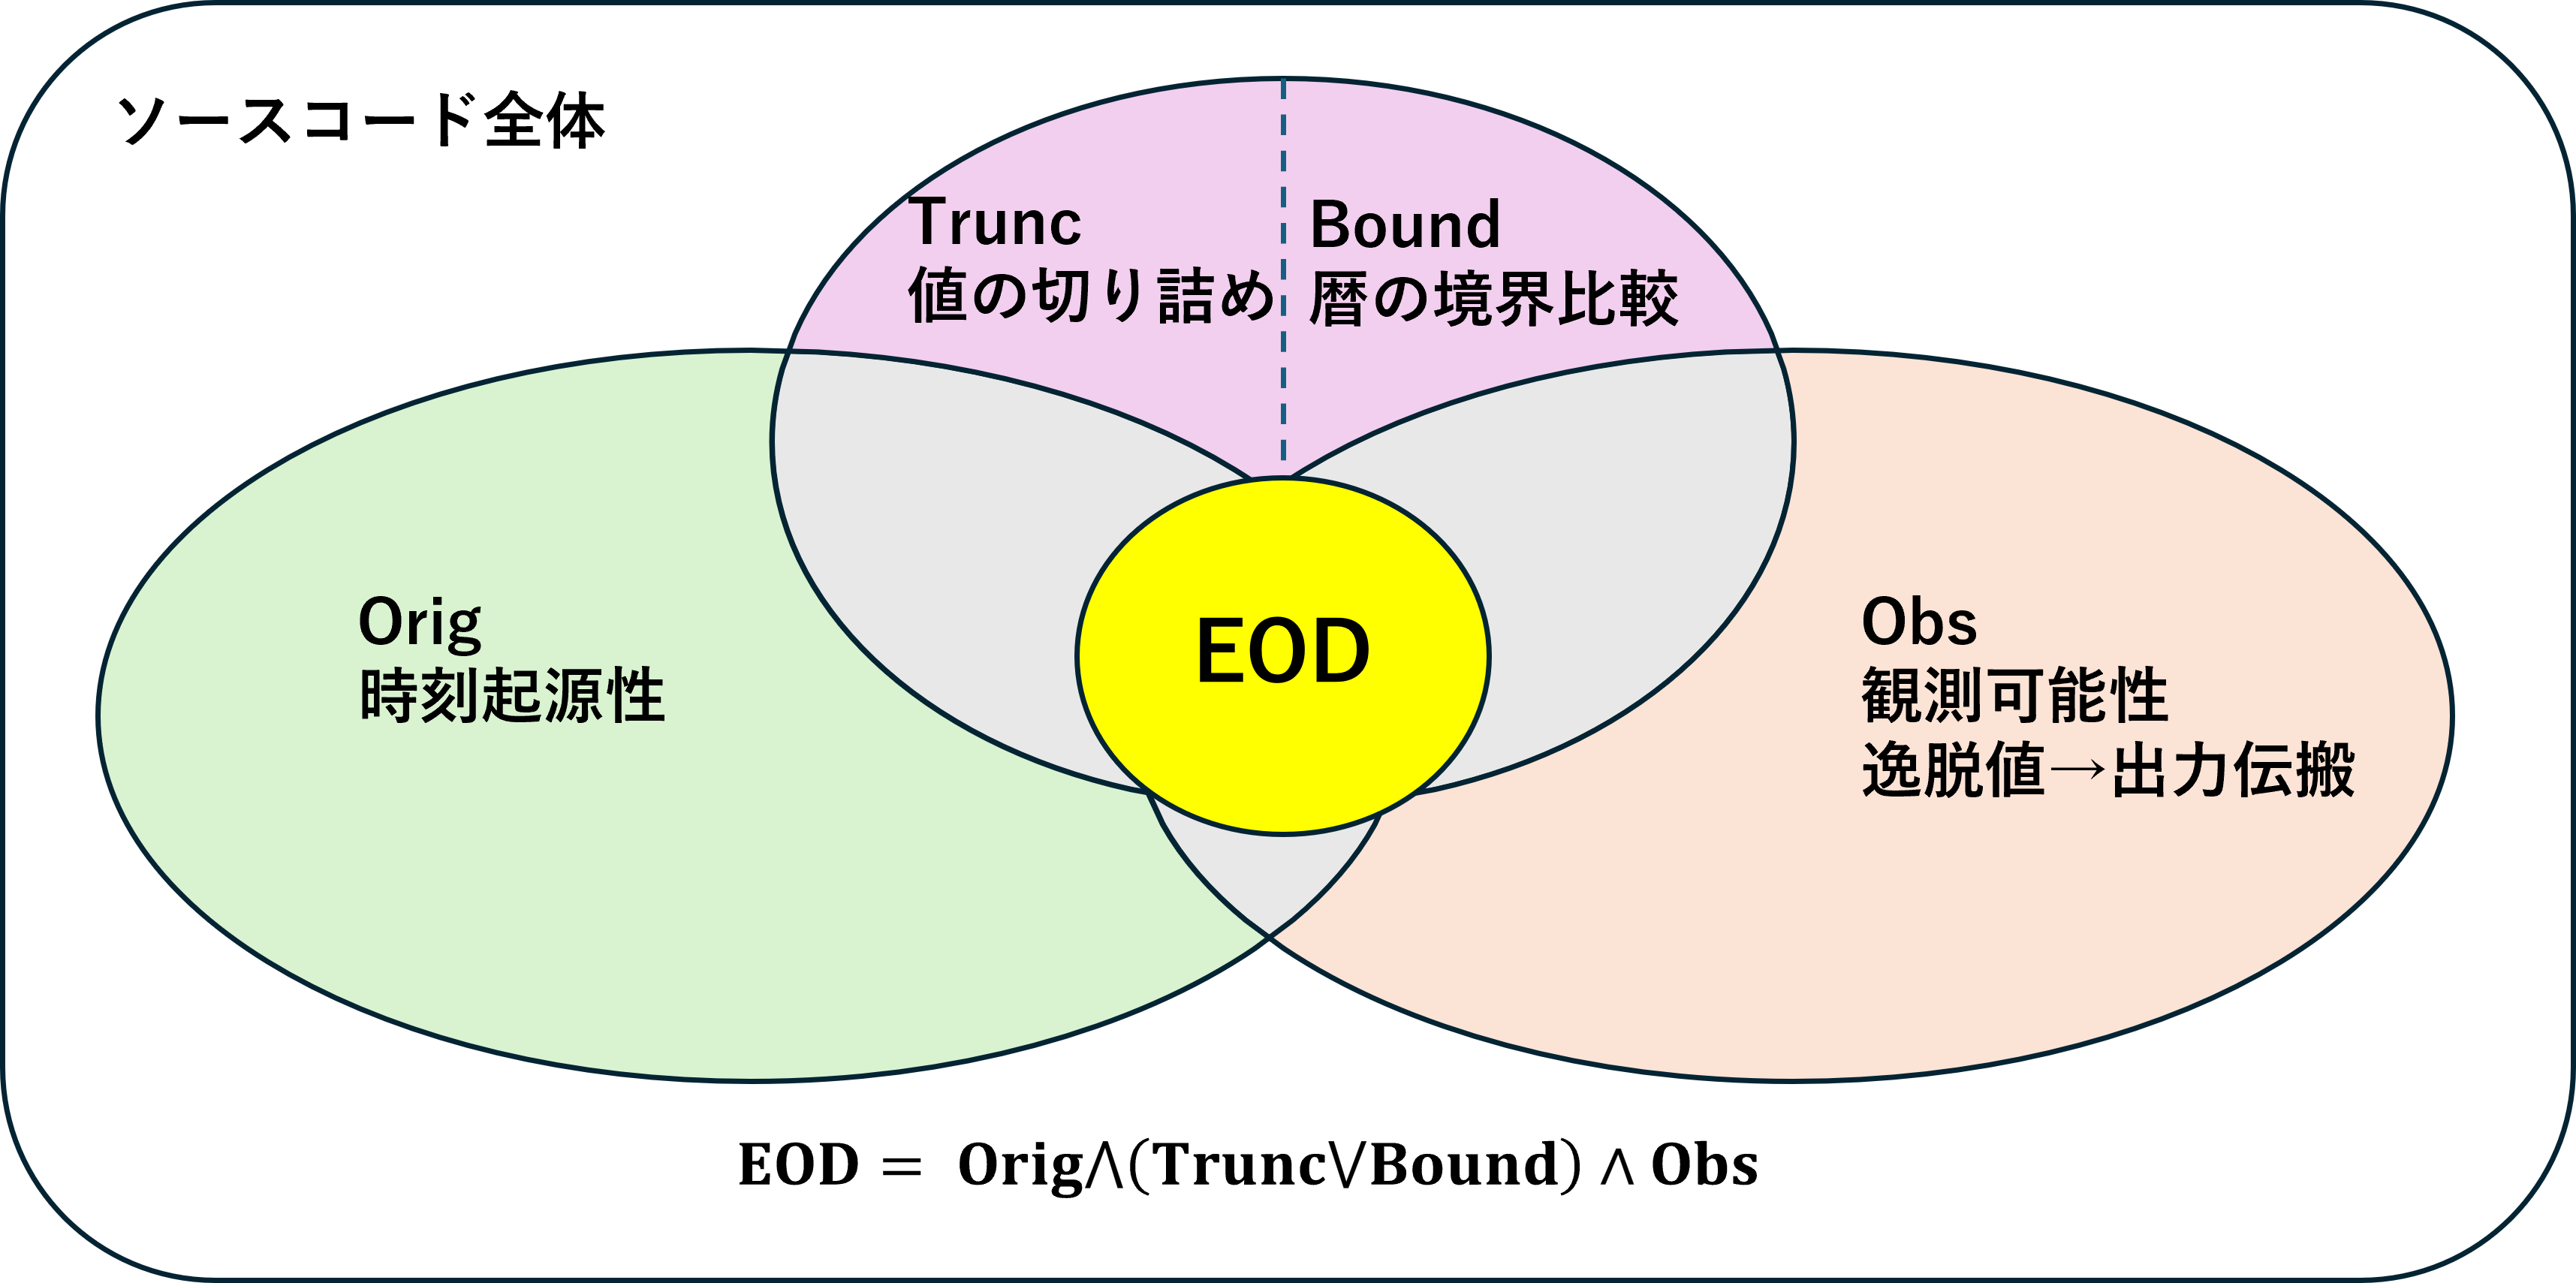
\includegraphics[width=\linewidth]{imgs/Figure2.1.png}
	\caption{エポックオーバーフロー欠陥（EOD）の構成}
	\ecaption{Structure of the Epoch Overflow Defect.}
	\label{fig:2.1}
\end{figure}

各述語の意図を述べる．$\mathrm{Orig}$は，検出対象を時刻意味論に依存する式に限定し，2038年問題とは無関係な一般的な整数オーバーフローを定義から排除するためのものである．論理和$\mathrm{Trunc} \lor \mathrm{Bound}$は，2038年問題の根本原因を「型幅に起因する値の切り詰め」と「コードに埋め込まれた暦境界」という二つの異なる類型に明確に分離している．いずれも環境の64ビット化（time\_t型の拡張など）のみでは解消されず，前者は代入や間接参照の過程で依然として型幅のミスマッチ（切り詰め）が発生するのに対し，後者は型幅に依存せず比較・評価ロジックそのものに起因して問題が存続するという性質の違いが，この分離の背景にある．最後に$\mathrm{Obs}$は，デッドコードや後続で上書きされる無害な値を欠陥から除外し，検出器の適合率を評価する際に有効となる．式\ref{eq:2.1}の関係を図\ref{fig:2.1}に図示する．

\subsubsection{二類型の実例}

式\ref{eq:2.1}の論理和部分，すなわち値の切り詰めと暦に関する境界値の評価について，実在のCコード（FreeBSD\cite{ref3}のdate系の時刻処理を単純化したもの）を用いて例示する．

\paragraph*{例1: 切り詰め型}

\begin{tcolorbox}[
	enhanced,
	breakable,
	colframe=black,
	colback=black!4,
	coltext=black,
	left=2mm,
	right=2mm,
	top=2mm,
	bottom=2mm,
	enlarge top by=4pt,
	enlarge bottom by=4pt,
	before skip=4pt,
	after skip=4pt,
]
\begin{verbatim}
static int domktime(struct tm *t, char type)
{
    time_t ret;
    ret = mktime(t);   /* 返り値型 time_t */
    return ret;        /* time_t -> int */
}
\end{verbatim}
\end{tcolorbox}

retはmktime()の返り値であり時刻要素から派生するため$\mathrm{Orig}$が成立する．return ret;においてtime\_t型の値をint型でreturnしている．64ビットtime\_t環境では32ビットのint型よりビット幅が広く，かつ2038年以降の時刻値は int の表現可能範囲に収まらないため，$\mathrm{Trunc}$が成立する．この返却値は呼び出し側の分岐処理などに利用され，上書きされることはないため，$\mathrm{Obs}$も成立する．本欠陥の原因はtime\_t型の幅ではなく，返り値の型指定の縮小にあるため，time\_t型を64ビット化しても問題として残留する．

\paragraph*{例2: 境界型}

\begin{tcolorbox}[
	enhanced,
	breakable,
	colframe=black,
	colback=black!4,
	coltext=black,
	left=2mm,
	right=2mm,
	top=2mm,
	bottom=2mm,
	enlarge top by=4pt,
	enlarge bottom by=4pt,
	before skip=4pt,
	after skip=4pt,
]
\begin{verbatim}
while ((ret = mktime(t)) == -1
       && t->tm_year > 68
       && t->tm_year < 138) {
    /* 失敗時に年を補正して再試行 */
}
\end{verbatim}
\end{tcolorbox}

t-\textgreater tm\_yearおよびmktime()の結果は時刻情報に起源を持つため，$\mathrm{Orig}$が成立する．定数138（tm\_yearは1900年起点ゆえ西暦2038年を表す）が暦的上限を表し，tm\_yearが138以上となる時刻でループ条件が偽となり補正処理に到達しないため$\mathrm{Bound}$が成立する．補正の有無は後続の時刻処理結果に影響するため$\mathrm{Obs}$も成立する．本欠陥の原因はコードに埋め込まれた「暦に関する知識」にあるため，time\_t型を64ビット化しても定数138が残る限り問題は解消されない．

これら二つの例は，いずれも単なる「64ビット化」では解消しない問題であるが，検出手法の観点からは大きな違いがある．例1は型システムに起因するため，静的な型情報から比較的容易に検出可能である．一方，例2は定数に込められた暦的な意味（セマンティクス）の解釈を要する．このことから，提案手法の適用範囲を以下のように決める．

\subsubsection{解ける範囲の画定}
\label{sec:解ける範囲の画定}

式\ref{eq:2.1}のうち，2038年問題につながる恐れのある$\mathrm{Orig} \land (\mathrm{Trunc} \lor \mathrm{Bound})$を満たす候補箇所をまずは検出し，$\mathrm{Obs}$の最終的な判定は人間のレビューに委ねる．そのレビューコストを削減するために候補集合の「適合率」を可能な限り高める方針とし，候補箇所の検出をLLMによって自動化し，最終判定を行う人間のレビューについてもLLMで支援することを提案する．$\mathrm{Obs}$の厳密な判定は一般に困難であるため（詳細は\ref{sec:妥当性への脅威}節で述べる），本稿では問題解決の完全な自動化は目指さず，問題を「機械的に絞り込める部分」と「人間が判断する部分」とに分割する．この方針のもとでは真の再現率は測定できないため，本稿では適合率を重視する．ただしモデル間の比較のため，\ref{sec:対象ソースコード}節にて述べるゴールドスタンダードに対する相対的な再現率およびF1スコアも併せて報告する．

\section{提案手法}

\begin{figure}[tb]
\begin{tcolorbox}[
	enhanced,
	colframe=black,
	colback=black!4,
	coltext=black,
	left=2mm,
	right=2mm,
	top=2mm,
	bottom=2mm,
	enlarge top by=4pt,
	enlarge bottom by=4pt,
	before skip=4pt,
	after skip=4pt,
]
\begin{verbatim}
指定したC言語のソースコードから，time_tが64ビットであっても発生する「2038年問題」の根本原因となる箇所を抽出し，以下に指定するJSON形式で出力せよ．出力はJSONのみとし，説明文を付けないこと．
【抽出条件】
・time_tが64ビット化されていても発生する「ロジック上の制限」を抽出すること．
・加えて，time_t型とint型やlong型のデータ間でオーバーフローやデータの切り詰めが発生する箇所を抽出すること．
・実装依存の場合は，その旨を問題の種類に明記すること．
・根本原因を修正することで不具合が発生しなくなる箇所は，抽出しないこと．
・添付のソースコード以外の情報は解答に利用しないこと．
【JSON形式】
{  "issues": [
    {
      "line": <問題となる命令文>,
      "type": <問題の種類>,
      "reason": <1文で理由>, 
      "fix": <1文で修正案>
    }
  ]
}
\end{verbatim}
\end{tcolorbox}
\caption{プロンプト}
\ecaption{Prompt.}
\label{fig:3.1}
\end{figure}

\begin{figure}[b]
	\centering
	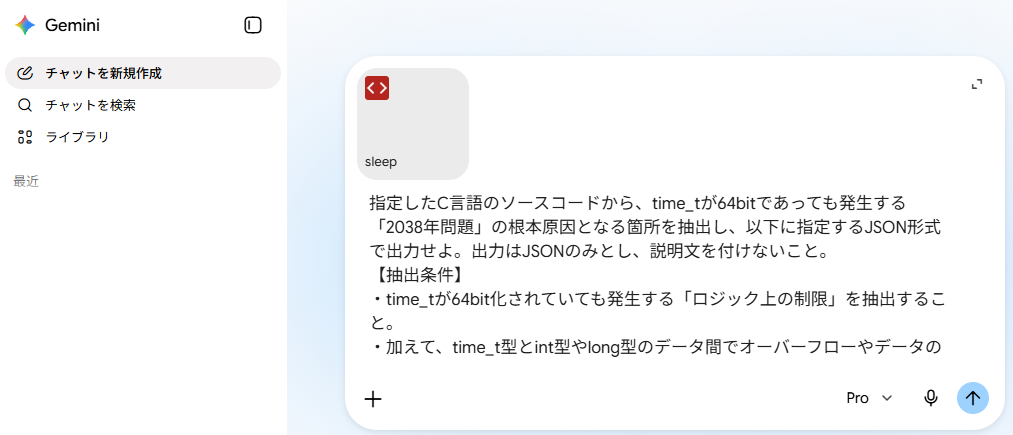
\includegraphics[width=\linewidth]{imgs/Figure3.2.png}
	\caption{Google Gemini 3.1 Proへの適用例}
	\ecaption{Application Example for Google Gemini 3.1 Pro.}
	\label{fig:3.2}
\end{figure}

\begin{figure}[b]
	\centering
	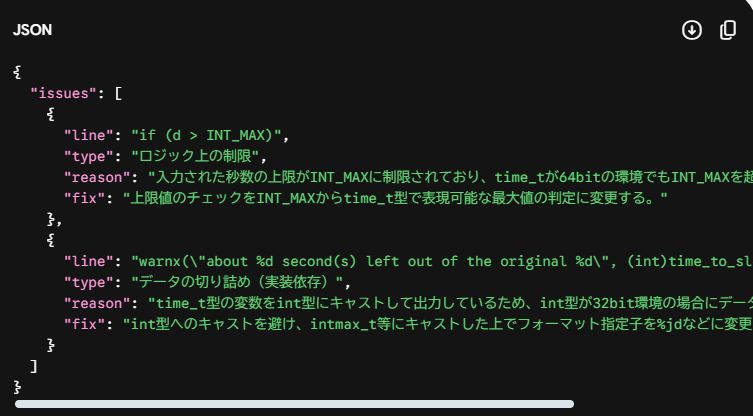
\includegraphics[width=\linewidth]{imgs/Figure3.3.png}
	\caption{適用結果の例}
	\ecaption{Examples of LLM Application Results.}
	\label{fig:3.3}
\end{figure}

前章で示した通り，2038年問題の解決には人間が判断する部分が残る．本研究ではこの部分にLLMを適用し，問題解決の省力化を目指した．近年のLLMは，自然言語による対話形式で多様な問いへの応答を生成できるだけでなく，プログラミング言語の解析においても実用レベルの精度を示すようになっている\cite{ref4,ref5}．本研究では，2038年問題の検出にLLMを適用することで，以下のメリットが得られることを期待している．

\begin{itemize}
	\item 修正が必要な箇所を簡単なプロンプトによって発見できる．
	\item 各データ型の実際のビット幅を仮定することなく，実装依存箇所についても自然言語の文脈を読み解いて発見できる．
	\item コンパイラ警告として顕在化しないロジック上の制約についても，コードの意味理解に基づいて指摘できる可能性がある．
\end{itemize}

\subsection{EODの検出手順}

LLMを活用したEODの検出手順は次のとおりである．最初に，専用アプリケーションやWebブラウザ経由で利用可能なLLMの中から，使用するモデルを選択する．本手法では，C言語ソースコードを1ファイルずつ入力し，個別に検出を各モデルにつき1回行う．選択したモデルのサービス画面において，図\ref{fig:3.1}のプロンプトを記述し，解析対象のC言語ソースコードを添付して処理を開始する．

なお，対象ソースコードは最大でも1ファイルあたり約1000行（概ね数千～1万トークン）であり，各LLMの最大コンテキスト長（最小のモデルでも128,000トークン以上）に十分収まる．このためファイルの分割や要約は不要であり，コンテキスト長に起因する入力の切り詰めや精度低下を，本実験では考慮しない．

図\ref{fig:3.2}にGoogle Gemini 3.1 Proでの実験の様子を，また図\ref{fig:3.3}にLLM適用結果の例を示す．

\subsection{LLM利用時の留意点}
\label{sec:LLM利用時の留意点}

一方で，LLMをソースコード解析に利用するにあたっては，以下の点に留意する必要がある．第一に，どのモデルを利用するかである．LLMの種類は急速に増加しており，モデル毎にコード理解能力や得意分野が異なる．第二に，どのプロンプトを与えるかである．プロンプト設計（プロンプトエンジニアリング）はLLMの応答品質を大きく左右する\cite{ref6}．第三に，モデルとプロンプトの組合せが適切かである．第四に，LLMの応答に内在する「揺らぎ」（確率的サンプリングや浮動小数点演算の非決定性に起因する応答のばらつき）をどう扱うかである\cite{ref7}．本稿ではこれらのうち主としてモデル選択の観点から比較評価を行う．

\section{評価実験}

\subsection{実験の概要}

本実験では，EODを含むことが事前にわかっている5本のC言語ソースコードを対象に，複数のLLMがどの程度の精度で該当箇所を検出できるかを評価する．プロンプトは全モデル共通とし，各モデルの出力結果を真陽性（TP）と偽陽性（FP）に分類して比較した．なお，\ref{sec:解ける範囲の画定}節で述べた「機械的に絞り込める部分」と「人間が判断する部分」への分割のうち，本実験で評価するのはLLMによって自動化できる候補検出の部分であり，人間が最終的に判断する部分は評価対象に含めない．

\subsection{対象ソースコード}
\label{sec:対象ソースコード}

対象ソースコードは，既報の研究で用いたFreeBSD13.2-RELEASE\cite{ref3}に含まれる以下の5本である．これらは時刻を扱う代表的なユーティリティであり，過去のコードレビューによりEODの箇所が同定されている．合計の真陽性数（ゴールドスタンダード，以降Ngold）は17箇所である．

\begin{itemize}
	\item sleep.c：sleepコマンドの実装．time\_t型の値をint型へキャストして表示する箇所を含む（EOD 2箇所）．
	\item tar.c：pax/tarアーカイバの実装．st\_mtimeをu\_long型にキャストして8進ASCII表現で書き出す箇所などを含む（EOD 2箇所）．
	\item cpio.c：cpioアーカイバの実装．tar.cと同様のキャスト箇所を含む（EOD 4箇所）．
	\item print.c：psコマンドの出力整形ロジック．tv\_secをint型変数secsへ代入する箇所6箇所とtime\_t型変数の演算結果をint型に代入する1箇所（EOD 7箇所）．
	\item vary.c：dateコマンドのオプション処理．mktime()のリトライ条件でtm\_yearを68～138に制限するロジックを含む（EOD 2箇所）．
\end{itemize}

\subsection{評価対象モデル}

本実験ではWebインタフェースもしくはアプリ経由で利用可能な以下の主要なLLMを比較対象とした．予備実験を行ったうえで，本稿の本評価では特に，Microsoft Copilot（Edgeブラウザ上でThink Deeperモードを有効化）, Google Gemini 3.1 Pro, Anthropic Claude Sonnet 4.6（Adaptive Thinkingモードを有効化）の3モデルを取り上げる．いずれも汎用LLMでありソースコード解析専用のチューニングは施していない．

\subsection{プロンプト}

前述の通り，図\ref{fig:3.1}に示したプロンプトを利用する．プロンプトは日本語で記述した．出力フォーマットをJSON\cite{ref8}に固定することで，自然言語の混入や表記の不統一といった出力形式の揺らぎを抑え，モデル間の機械的な比較を可能とするよう工夫した．近年のLLMはJSON形式での構造化出力機能が標準的にサポートされており\cite{ref9}，パースエラーを防げる利点がある．ただし，これは出力形式を一定に保つだけであり，\ref{sec:LLM利用時の留意点}節で述べた応答内容の揺らぎそのものを解消するわけではない．

またプロンプトにより，式\ref{eq:2.1}のEODを求めるため，式の各項目と，プロンプトを対応させる必要がある．式\ref{eq:2.1}とプロンプトとの対応関係を表\ref{tab:4.1}に示す．

\begin{table}[bt]
	\centering
	\caption{式\ref{eq:2.1}とプロンプトの対応関係}
	\ecaption{Eq. \ref{eq:2.1}-Prompt Mapping.}
	\label{tab:4.1}
	\begin{tabular}{|l|p{5cm}|}
\hline
\textbf{式\ref{eq:2.1}の項目} & \textbf{プロンプトでの表現} \\
\hline
$\mathrm{Orig}$ & 指定したC言語のソースコードから，time\_tが64ビットであっても発生する「2038年問題」の根本原因となる箇所を抽出し， \\
\hline
$\mathrm{Trunc}$ & time\_t型とint型やlong型のデータ間でオーバーフローやデータの切り詰めが発生する箇所を抽出すること． \\
\hline
$\mathrm{Bound}$ & time\_tが64ビット化されていても発生する「ロジック上の制限」を抽出すること． \\
\hline
$\mathrm{Obs}$ & 実装依存の場合は，その旨を問題の種類に明記すること． \\
\hline
\end{tabular}
\end{table}

ここで，$\mathrm{Obs}$（観測可能性）に対して実装依存の明記を求めているのは，LP64やLLP64といったデータモデルの違いにより，特にlong型の変数においてエポックオーバーフロー欠陥（EOD）がデータフロー上で問題として顕在化（観測）するか否かが分かれるためである．LLMに実装依存の文脈を意識させることで，環境ごとの観測可能性を制御する意図がある．

\subsection{評価指標}

各モデルの応答について，事前に同定されたEOD箇所と一致する指摘を真陽性（True Positive，TP），それ以外の指摘のうちEODに該当しないものを偽陽性（False Positive，FP）として分類した．これらをもとに，適合率（Precision = TP / (TP+FP)），再現率（Recall = TP / Ngold），およびF1スコア（= 2·Precision·Recall / (Precision+Recall)）を算出した．ここでNgoldはゴールドスタンダードのEOD箇所数である．なお，\ref{sec:解ける範囲の画定}節で述べた通り真の再現率は算出できないため，本実験におけるRecallは，事前に同定されたゴールドスタンダードNgoldに対する相対的な再現率を意味する．

\section{実験結果}

各ソースコードに対する各モデルのTP数とFP数を「TP / FP」の形式で表\ref{tab:5.1}に，それらから算出したPrecision，Recall，F1スコアを表\ref{tab:5.2}に示す．Google Gemini 3.1 Proが16箇所のEOD箇所を検出（再現率0.94）し，かつ偽陽性数も最も少なかった．Claude Sonnet 4.6は13/17箇所を検出（再現率0.76）し，偽陽性は3箇所であった．Copilotは12/17箇所を検出（再現率0.71）し，特にprint.cにおける複数のtv\_sec代入箇所の検出を取りこぼした．総合的なF1スコアではGoogle Gemini 3.1 Proが0.94と最も高く，Claude Sonnet 4.6が0.79，Copilotが0.73であった．

Google Gemini 3.1 ProのF1スコアが0.94であったという結果は，現時点で同モデルの総合的な検出精度の高さを示している．対象箇所を漏れなく指摘する能力に優れているだけでなく，誤った箇所を指摘する偽陽性も最小限に抑えられており，実用性の高い結果であった．

\begin{table}[bt]
	\centering
	\caption{各モデルの検出結果}
	\ecaption{Detection results per model.}
	\label{tab:5.1}
	\begin{tabular}{|l|c|c|c|c|}
\hline
\textbf{ソース} & \textbf{Ngold} & \textbf{Copilot} & \begin{tabular}{c} \textbf{Gemini} \\ \textbf{3.1 Pro} \end{tabular} & \begin{tabular}{c} \textbf{Sonnet} \\ \textbf{4.6} \end{tabular} \\
\hline
sleep.c & 2 & 2 / 0 & 2 / 0 & 2 / 0 \\
\hline
tar.c   & 2 & 2 / 1 & 2 / 1 & 2 / 2 \\
\hline
cpio.c  & 4 & 4 / 1 & 4 / 0 & 3 / 1 \\
\hline
print.c & 7 & 2 / 1 & 6 / 0 & 4 / 0 \\
\hline
vary.c  & 2 & 2 / 1 & 2 / 0 & 2 / 0 \\
\hline
合計    & 17 & 12 / 4 & 16 / 1 & 13 / 3 \\
\hline
\end{tabular}
\end{table}

\begin{table}[bt]
	\centering
	\caption{各モデルの検出精度}
	\ecaption{Detection precision per model.}
	\label{tab:5.2}
	\begin{tabular}{|l|c|c|c|}
\hline
\textbf{指標} & \textbf{Copilot} & \textbf{Gemini 3.1 Pro} & \textbf{Sonnet 4.6} \\
\hline
Precision & 0.75 & 0.94 & 0.81 \\
\hline
Recall    & 0.71 & 0.94 & 0.76 \\
\hline
F1        & 0.73 & 0.94 & 0.79 \\
\hline
\end{tabular}
\end{table}

\section{議論}

\subsection{実験結果の総括}

個別のソースコードについて見ると，sleep.c，tar.c，vary.cでは全モデルがゴールドスタンダードを完全に検出した．tar.cでは全モデルが2箇所のEODを検出したが，関数定義そのもの（150行目のul\_oct）を誤って指摘する偽陽性が発生した．print.cはtv\_sec値をint型変数へ代入する箇所が複数（547行目，571行目，574行目，585行目，588行目，604行目）あり，モデル間の差が最も顕著であった．Copilotは2/7箇所しか検出できなかったのに対し，Google Gemini 3.1 Proは6/7箇所を検出した．Claude Sonnet 4.6は4/7箇所を検出した．

これらの結果は，時刻値への直接的な操作は全モデルが安定して検出できる一方，間接参照を付す箇所ではデータフロー追跡能力の差がモデル間の差として現れることを示唆している．以下では，LLMによる問題の検出に影響するソースコード上の特徴を整理する．

まず，sleep.c，tar.c，vary.cで全モデルが検出した箇所は，時刻データに対する直接的な比較・キャスト・ビット演算や戻り値の型不一致など，いずれも確認範囲が限定されるため比較的検出が容易であると推察される．

tar.cでのst\_mtimeに対するキャスト処理の箇所については，コンパイルスイッチにより，対象処理の有効・無効を切り替えている．このコンパイルスイッチの解釈やマクロ展開の捉え方の違いが，LLM間での偽陽性（FP）の指摘傾向の差（Sonnet 4.6のみFPが2箇所など）に影響したのではないかと推察している．図\ref{fig:6.1}にtar.cで偽陽性の原因と考えられる，st\_mtimeを保持する箇所のコード片を示す．

\begin{figure}[tb]
	\centering
	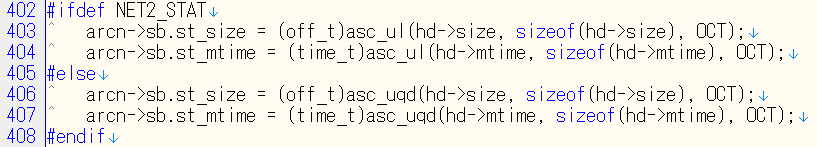
\includegraphics[width=\linewidth]{imgs/Figure6.1.png}
	\caption{tar.cで偽陽性の原因と考えられるコード片}
	\ecaption{Suspected False-Positive Code in tar.c.}
	\label{fig:6.1}
\end{figure}

なお，図\ref{fig:3.1}のプロンプトは式\ref{eq:2.1}の各述語を完全に表現できているわけではない．$\mathrm{Orig}$については「2038年問題の根本原因」という表現にとどまり，値が時刻意味論に由来することを明示的に確認させていない．また$\mathrm{Obs}$は，\ref{sec:外部への観測可能性}節ではコンパイルスイッチによる除外までを含む広い概念であるのに対し，今回のプロンプトでは「実装依存の場合はその旨を明記する」という指示としてしか与えておらず，コンパイルスイッチで無効化される箇所を検出対象から外す指示を明示していない．この$\mathrm{Obs}$の部分的な表現が，tar.cにおけるコンパイルスイッチに依存したFPを生んだ一因ではないかと考えられる．

ul\_oct関数定義そのものに対する指摘は偽陽性ではあるが，陽性の指摘箇所が，ul\_oct関数呼出し時の引数内のキャスト処理でみられることから，検出対象として挙がったものと推察する．

cpio.cについては，Claude Sonnet 4.6で1件検出ができなかった箇所があった．この部分は，time\_t型の値の演算結果を，time\_t型の変数に代入する処理であり，代入処理には問題は無いが，演算の中に32ビットの値を前提としたシフト演算がある．問題が起きるか否かは文脈により異なる部分であり，検出するか否かは判断の分かれるものと考えられる．

なお，cpio.cでは，Claude Sonnet 4.6とCopilotで，FPを1つずつ記録している．これは前述の検出漏れの箇所とは別に，時刻情報を8ビットずつ切り出して別変数に保存する処理を指摘したものである．ここが2038年問題につながるか否かは，別ファイルで定義されているマクロにも依存するため，人による判断が必要となる．本実験のプロンプトでは与えたファイル以外の情報を検出に用いないよう指示しているため，この箇所を検出しなかったGoogle Gemini 3.1 Proの挙動は，むしろプロンプトに忠実な結果と解釈できる．したがって，当該箇所の検出をFPとすべきか否かは，ゴールドスタンダードの定義に依存する事例であり，\ref{sec:妥当性への脅威}節で述べるゴールドスタンダードの主観性に関する脅威の具体例と位置づけられる．

また，検出結果に差が大きかったprint.cには，構造体メンバの参照，代入，演算に関する処理が6箇所存在している．このうち5箇所を検出したのが，Google Gemini 3.1 Proであり，1箇所のみ検出したのがCopilotである．Claude Sonnet 4.6は，6箇所中3箇所検出しており，ここで結果に差が出ている．この構造体メンバはポインタ変数を経由してtime\_t型の値にアクセスするようになっており，データへの間接参照を行う処理については，LLMの特徴によって検出結果の差が大きく出るものと推察している．図\ref{fig:6.2}にprint.cで問題を検出した，構造体メンバの例を示す．

\begin{figure}[tb]
	\centering
	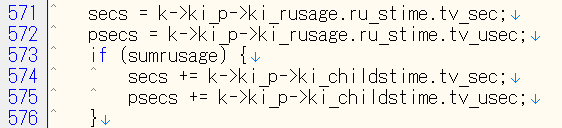
\includegraphics[width=\linewidth]{imgs/Figure6.2.png}
	\caption{print.cで問題となるコード片}
	\ecaption{The problematic code snippet in print.c.}
	\label{fig:6.2}
\end{figure}

print.cの7箇所目の問題点は，time\_t型の値の演算結果を，直接int型変数に代入する処理であり，これについてはすべてのLLMで正しく検出している．

まとめると，LLMを用いた本手法で検出率を上げるには，以下の注意点に従うと良いと考える．
\begin{itemize}
	\item コンパイルスイッチがあるソースコードについては，どのコードが有効になるかをプロンプト内で明示的に指示すること．
	\item データの間接参照についてはモデル間で検出結果に差が出ることから，複数のLLMでの複数回の実験により，問題箇所の推定を行うこと．
\end{itemize}
今回はCopilotの見落としが最も多かったが，サンプル数が少なく，この結果のみで性能を論じることはできない．

\subsection{従来手法との比較}

筆者らはこれまでに2038年問題に対する二つのアプローチを報告してきた．第一は，2019年に組込み機器の実製品開発において行った対応事例である\cite{ref10}．この事例では，time\_t型を32ビットのまま維持しつつ，UNIXエポックを28年後に設定する（具体的には1998年1月1日を新たな起点とする）ことで，運用上必要となる時刻範囲を確保し，2066年まで「延命」する手法を採用した．第二は，2023年に報告したtime\_t型を64ビット化した際に修正が必要となる箇所をコンパイラ警告の差分から抽出する手法である\cite{ref11}．この手法では，64ビット化前後でコンパイラから出力される警告（型の不整合や暗黙的キャストに関する警告）の差分を取り，かつ意図的なキャストが明示されている箇所を除外することで修正候補箇所を絞り込む．

しかし，いずれの手法も限界を持つ．延命策はあくまで暫定的対応であり，対応期限を先送りするに過ぎない．コンパイラ警告の差分による検出は，警告として顕在化する型不整合は検出できるが，u\_long等への明示的キャストの裏に隠されたロジック上の制約（例えば32ビット幅を前提とした条件式）までは検出できない．

その他プログラムスライシングやデータフロー解析\cite{ref12}は理論的には最も有力な手段だが，大規模なソフトウェアに適用するには解析コストが大きく，セマンティクスにより問題の有無を人間が判断する必要は変わらず存在する．

2038年問題に対しては，筆者ら以外の研究も報告されている．星名らは，time\_t型が32bitを超える（64ビット化された）環境においてもなお残存しうる2038年問題に着目し，その検出手法を提案している\cite{ref13}．一方，矢吹らは，32bit Linux環境を対象に，時刻同期プロトコル内で時刻変換を行うことで2038年問題に対処する手法を提案している\cite{ref14}．

本稿で提案したLLMによる検出手法は，人間による判断コストを低減させる．利用モデルによる結果の不安定さは課題だが，複数モデル・複数回の試行を総合することで緩和できると考える．これにより，従来手法より問題検出の効率を向上させることが期待できる．

\subsection{妥当性への脅威}
\label{sec:妥当性への脅威}

式\ref{eq:2.1}で表現したモデルの妥当性，および本モデルの位置づけに対する脅威について，以下に議論する．

本モデルでは，2038年問題の具体的な発生要因として，これまでの筆者の研究調査に基づき「値の切り詰め（$\mathrm{Trunc}$）」および「暦に関する境界値の評価（$\mathrm{Bound}$）」の二つを対象としている．しかし，これらは主要な要因として抽出したものであり，2038年問題を引き起こすあらゆる原因を網羅できているとは限らない．例えば，特定のミドルウェアやサードパーティ製ライブラリ内での暗黙的な型変換，あるいはシリアライズ処理に起因するデータ構造上の不整合など，本モデルの想定外の形式で問題が顕在化する可能性（偽陰性の発生）が残されている．

また，モデル中の「外部への観測可能性（$\mathrm{Obs}$）」は，検出されたコード上の問題が実際にシステムの不具合として表面化するかを評価する上で重要な指標である．しかし，あるプログラムの実行経路において特定の状態が外部に観測可能か否かを厳密に判定する問題は，一般に「停止問題」\cite{ref15}と同様に決定不能問題に帰着する．したがって，実際の検出手法において$\mathrm{Obs}$を完全かつ厳密に計算することは理論上不可能であり，静的・動的解析（例：汚染経路解析や限定的なシンボリック実行など）\cite{ref16}による近似に頼らざるを得ないと考える．この近似の精度が，検出結果の妥当性に直接影響を与える脅威がある．

以上の脅威に基づき，本研究における式\ref{eq:2.1}は，2038年問題の発生条件を完全に記述した「厳密な定義」ではなく，検出アプローチを体系化し，現実的な解析範囲を定めるためのヒューリスティックな概念的・運用的モデルとして位置づけるのが妥当である．今後は，実験評価を通じて未知の要因をフィードバックしモデルを拡張すること，および$\mathrm{Obs}$の現実的な近似手法の洗練を図ることが課題となる．

さらに，本実験の内的妥当性に関わる脅威として，ゴールドスタンダード（17箇所）の同定が筆者らの過去のコードレビューに基づく主観的判断に依拠している点が挙げられる．あるコード片に対してEODに該当すると判定すること自体がプログラムのセマンティクスに依存するため，境界的な事例では誰が判断したかによって解釈が分かれ得る．また，各モデルの応答をTP／FPに分類する際も同一のゴールドスタンダードを基準とするため，ゴールドスタンダードに誤りや見落としがあれば，適合率・再現率の双方が系統的に偏る恐れがある．この脅威を低減するには，複数のレビュー者による独立な判定とその一致度に基づくゴールドスタンダードの構築や，EOD該当性の判定基準を明文化したうえでの再検証が望ましい．

また，評価に使用したデータセット\footnote{\url{https://github.com/hide-work/y2038-llm-dataset}にて本実験で用いたデータセットを公開している．}が5ファイル17箇所と小規模であり，より大規模なソースコード群では検出精度が変動しうるため，一般化可能性にはさらなる検証が必要である．また，本実験は各モデルにつき1回の試行に基づく結果であり，\ref{sec:LLM利用時の留意点}節で述べた応答の揺らぎの影響は評価していない．さらに，結果は使用したLLMの特定のバージョンに依存し，基盤モデルの更新や確率的な非決定性により同一条件下でも再現されない可能性がある．したがって本節の数値は速報的な位置づけであり，複数回試行による再現性・ロバスト性の検証は今後の課題である．

\section{おわりに}

本研究では，今後到来する2038年問題の対策として，ソースコード中から潜在的な問題箇所を効率的に検出するための手法について検討を行った．2038年問題の発生メカニズムを体系化し，時刻起源（$\mathrm{Orig}$），値の切り詰め（$\mathrm{Trunc}$），暦に関する境界値の評価（$\mathrm{Bound}$），および外部への観測可能性（$\mathrm{Obs}$）の論理式として表現する概念的モデルを提案した．さらに，本モデルに基づく問題箇所の識別能力を検証するため，大規模言語モデル（LLM）を用いた評価実験を行い，提案モデルの有用性とLLMによる検出の可能性を示した．

今後の課題としては，提案モデルおよびLLMによる検出精度のさらなる定量的な評価と改善が挙げられる．今後は，実際に$\mathrm{Trunc}$や$\mathrm{Bound}$の不具合を含むOSSのコード断片を広く収集し，評価用のゴールドスタンダードを拡充する．この拡充したデータセットを用いてLLMのプロンプトエンジニアリングやファインチューニング等の最適化を図り，より多様なコードパターンに対しても高精度に2038年問題箇所を特定できるアプローチの確立を目指す．また，本実験ではLLMによる候補検出の精度のみを評価しており，LLMによる支援を加えた人間のレビューを組み合わせたワークフロー全体でのレビューコスト削減効果の検証も行いたい．

\begin{thebibliography}{99}

\bibitem{ref1}
IEEE: The Open Group Base Specifications Issue 7, 2018 edition / IEEE Std 1003.1-2017, IEEE (2018).

\bibitem{ref2}
ISO: ISO/IEC 9899:2024 Information technology -- Programming languages -- C, International Organization for Standardization (2024).

\bibitem{ref3}
The FreeBSD Project: FreeBSD 13.2-RELEASE Release Notes (2023).

\bibitem{ref4}
Chen, M., et al.: Evaluating Large Language Models Trained on Code, arXiv preprint arXiv:2107.03374 (2021).

\bibitem{ref5}
Jain, N., et al.: LiveCodeBench: Holistic and Contamination Free Evaluation of Large Language Models for Code, arXiv preprint arXiv:2403.07974 (2024).

\bibitem{ref6}
Liu, P., et al.: Pre-train, Prompt, and Predict: A Systematic Survey of Prompting Methods in Natural Language Processing, ACM Computing Surveys, Vol. 55, No. 9, Article 195 (2023).

\bibitem{ref7}
Song, Y., Wang, G., Li, S., Lin, B. Y.: The Good, The Bad, and The Greedy: Evaluation of LLMs Should Not Ignore Non-Determinism, arXiv preprint arXiv:2407.10457 (2024).

\bibitem{ref8}
Bray, T.: The JavaScript Object Notation (JSON) Data Interchange Format, RFC 8259, IETF (2017).

\bibitem{ref9}
OpenAI: Structured model outputs, \url{https://developers.openai.com/api/docs/guides/structured-outputs} (参照 2026-06-15).

\bibitem{ref10}
大江秀幸, 安藤友康, 松下誠, 井上克郎: 組込み機器開発における2038年問題への対応事例, デジタルプラクティス, Vol. 10, No. 3 (2019).

\bibitem{ref11}
大江秀幸, 松下誠, 井上克郎: コンパイラー警告を利用したデータ型変更時の影響範囲確認方法の提案, 情報処理学会研究報告, Vol. 2023-SE-215, No. 4, pp. 1-8 (2023).

\bibitem{ref12}
Weiser, M.: Program Slicing, IEEE Transactions on Software Engineering, Volume 10, Issue 4, pp. 352-357 (1984).

\bibitem{ref13}
星名藍乃介, 穐山空道, 上原哲太郎: 32bitを超えるtime\_t型を持つ環境における2038年問題とその検出, 情報処理学会論文誌, Vol. 65, No. 9, pp. 1387-1398 (2024).

\bibitem{ref14}
矢吹潤, 岡部亮, 堀井圭祐, 外山正勝: 時刻同期プロトコル内の時刻変換による32bit Linuxの2038年問題対策, FIT2019講演論文集第1分冊, pp. 151-152 (2019).

\bibitem{ref15}
Sipser, M. (渡辺治, ほか訳): 計算理論の基礎 [原著第3版] 2. 計算可能性の理論, 共立出版 (2023).

\bibitem{ref16}
Schwartz, E. J., Avgerinos, T., Brumley, D.: All You Ever Wanted to Know about Dynamic Taint Analysis and Forward Symbolic Execution (but Might Have Been Afraid to Ask), Proc. IEEE Symposium on Security and Privacy, pp. 317-331 (2010).

\end{thebibliography}

\end{document}
